\documentclass[aspectratio=169]{beamer}
% \documentclass{beamer}

\usetheme{metropolis}
\usepackage[T1]{fontenc}
\usepackage{microtype}
\usepackage{booktabs}
\usepackage{float}
\usepackage{amsmath}
\usepackage{mathtools}
\usepackage{graphicx}
\usepackage{tabularray}
\usepackage{amssymb}
\usepackage{csquotes}
\usepackage{adjustbox}
\usepackage{hyperref}
\usepackage[justification=centering]{caption}

% --- Bibliography setup ---
\usepackage[
  backend=biber,
  style=authoryear,
  maxcitenames=2,
  uniquename=false,
  giveninits=true
]{biblatex}

\addbibresource{references/references.bib}
\title{Revisiting Link Prioritization for Efficient~Traversal in Structured Decentralized Environments}
\date{\today}
\author{Ruben Eschauzier, Ruben Taelman, Ruben Verborgh}
\institute{Department of Electronics and Information Systems, Ghent University – Imec}

\begin{document}

\maketitle

% NOTES:
%   Take more time to justify why decentralized environments, the use-case is good but:
%       - Mention how its only one of the use-cases
%       - Explain it more how decentralized matters with more anecdotes
%       - Transition from centralized to link traversal doesn't make any goddamn sense
%       - Why do we use documents? Why not sparql endpoints? Documents are very unexpressive allowing flexible data representation without large server cost.
%       - User in the loop privacy controls instead of granular, once data is in centralized storage its difficult to get it out.
%       - Maybe remove the slide talking about centralized querying
%       - Document serving of resources is less expressive (can answer less types of questions, just what is in the document)
%         becomes less expensive per level of granularity fine-grained access control

\begin{frame}{The Need for Decentralized Personal Data Storage}
    \begin{columns}[T] % T aligns columns at the top
        % Left column: Image
        \begin{column}{0.6\textwidth} % Adjust width as needed
            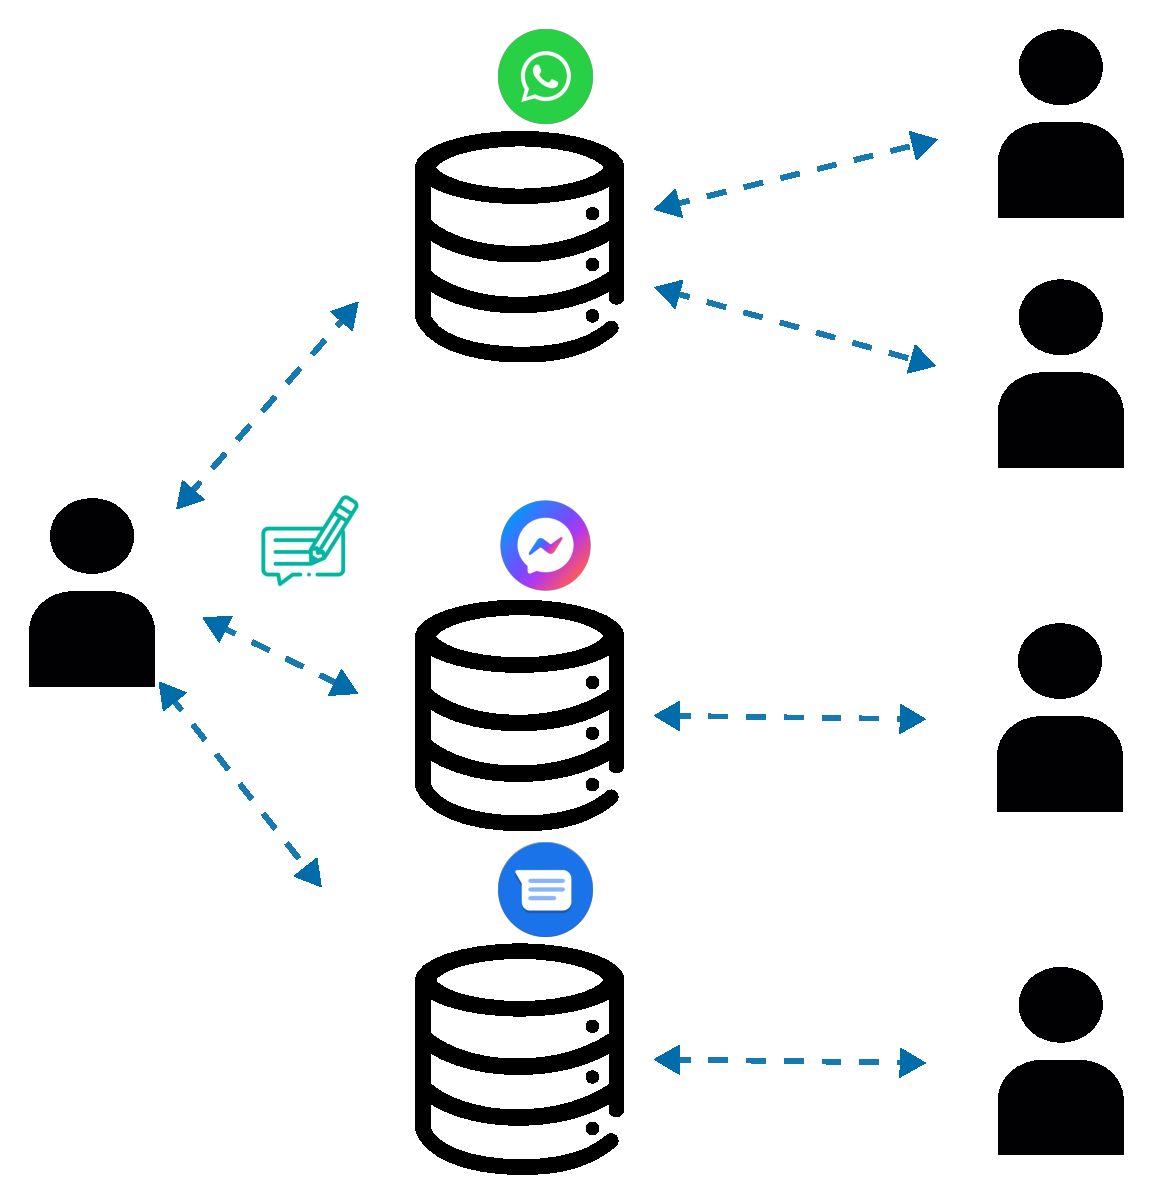
\includegraphics[width=.85\linewidth]{images/current-bad-message-situation.pdf} % replace with your image file
        \end{column}

        % Right column: Text
        \begin{column}{0.4\textwidth} % Adjust width as needed
            \begin{itemize}
                \item Each application has its own data
                \item Stifles innovation
                \item Causes vendor lock-in
            \end{itemize}
        \end{column}
    \end{columns}
\end{frame}


\begin{frame}{The Need for Decentralized Personal Data Storage}
    \begin{columns}[T] % T aligns columns at the top
        % Left column: Image
        \begin{column}{0.6\textwidth} % Adjust width as needed
            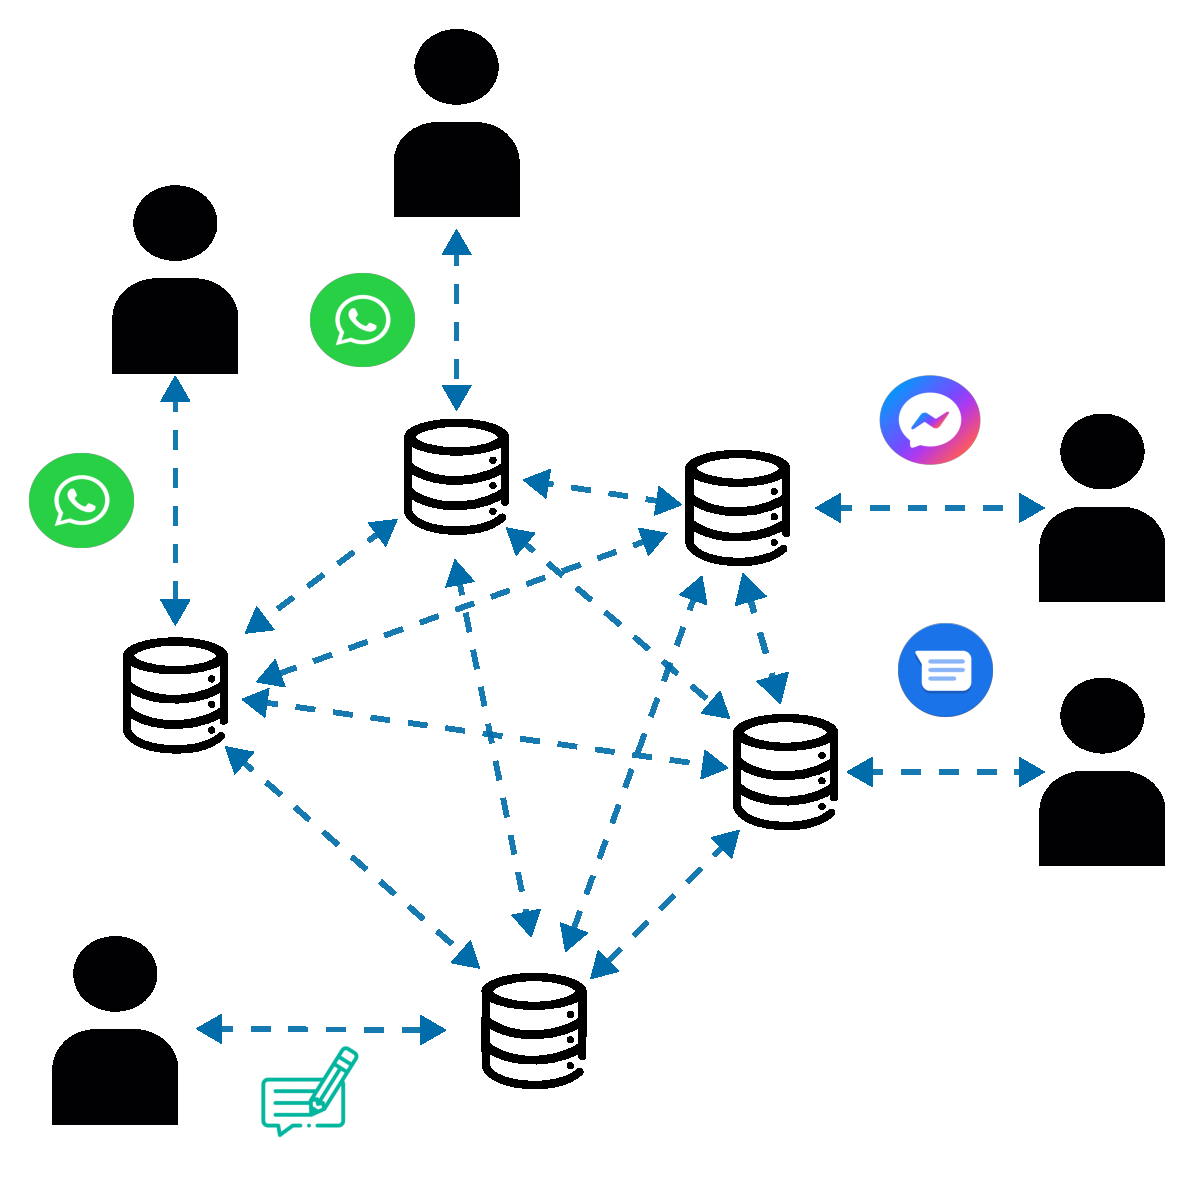
\includegraphics[width=.9\linewidth]{images/decentralized-message-storage.pdf} % replace with your image file
        \end{column}

        % Right column: Text
        \begin{column}{0.4\textwidth} % Adjust width as needed
            \begin{itemize}
                \item Each application uses common data storage
                \item Easy to switch vendors
                \item Promotes innovation
            \end{itemize}
        \end{column}
    \end{columns}
\end{frame}

\begin{frame}{The Problem with Centrally Aggregating and Querying}
    \begin{columns}[T] % T aligns columns at the top
        % Left column: Image
        \begin{column}{0.6\textwidth} % Adjust width as needed
            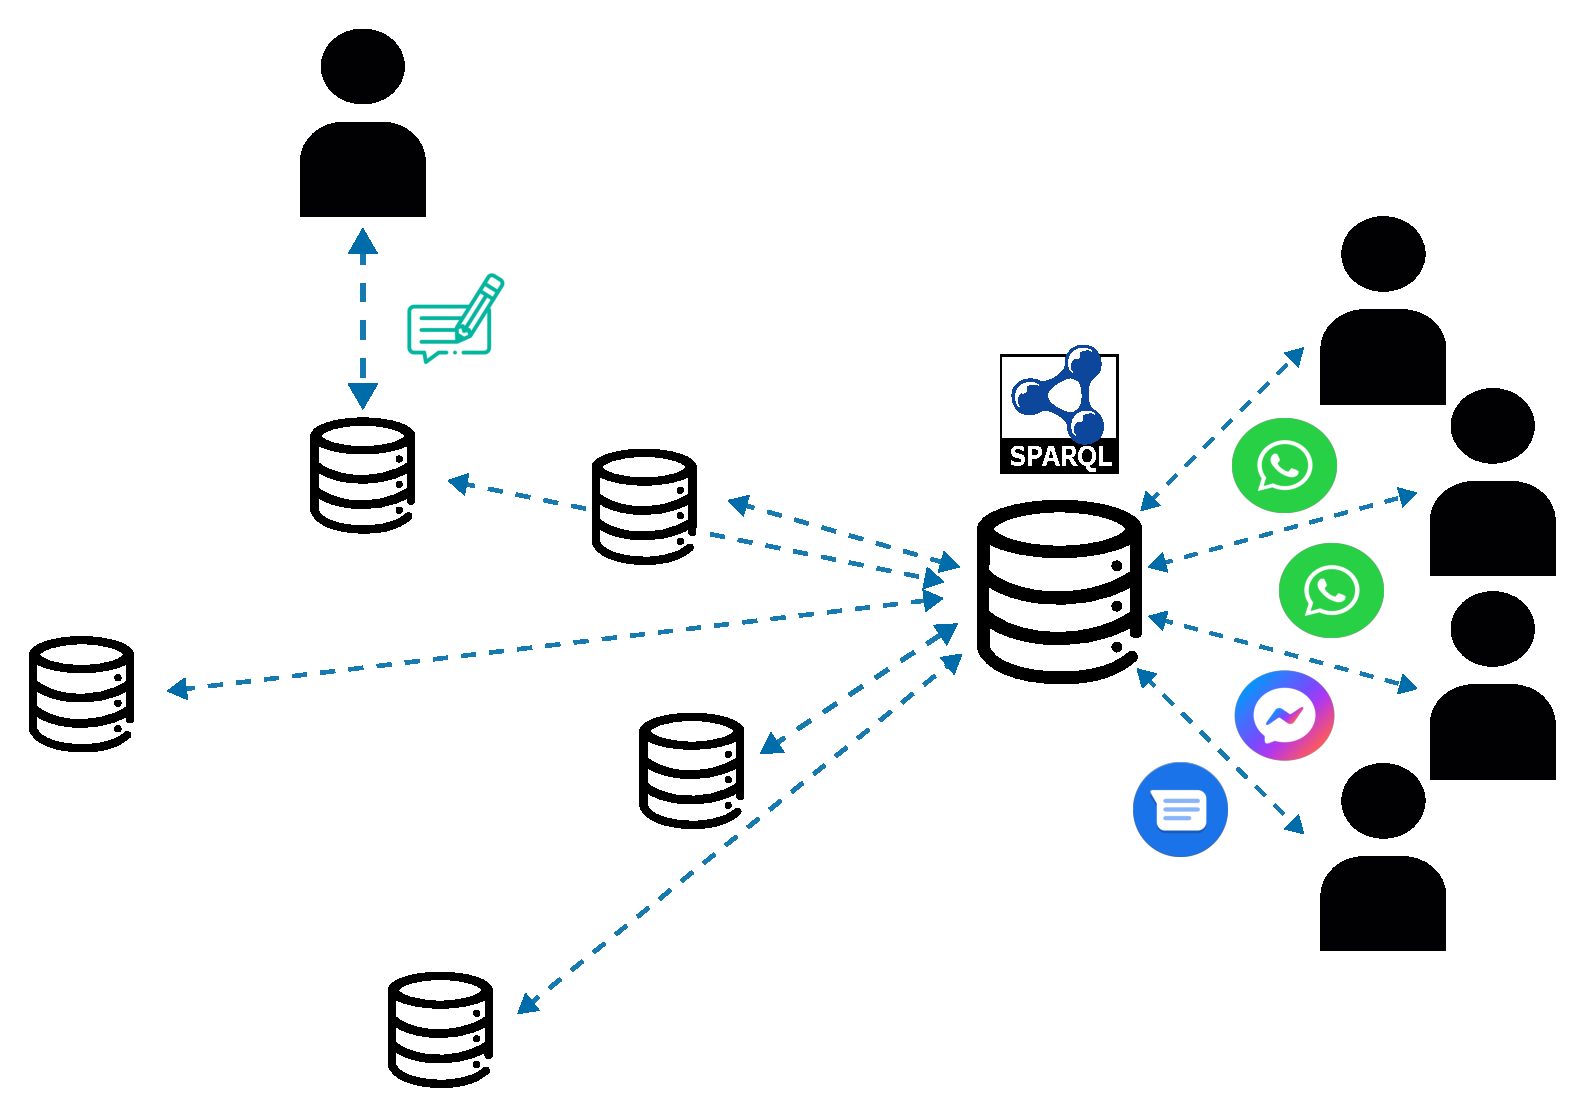
\includegraphics[width=\linewidth]{images/centralize-personal-data-stores.pdf} % replace with your image file
        \end{column}

        % Right column: Text
        \begin{column}{0.4\textwidth} % Adjust width as needed
            \begin{itemize}
                \item Why not aggregate data and query it?
                \item Difficult in case of personal data due to privacy concerns
            \end{itemize}
        \end{column}
    \end{columns}
\end{frame}

\begin{frame}{The Problem with Centrally Aggregating and Querying}
    \begin{columns}[T] % T aligns columns at the top
        % Left column: Image
        \begin{column}{0.6\textwidth} % Adjust width as needed
            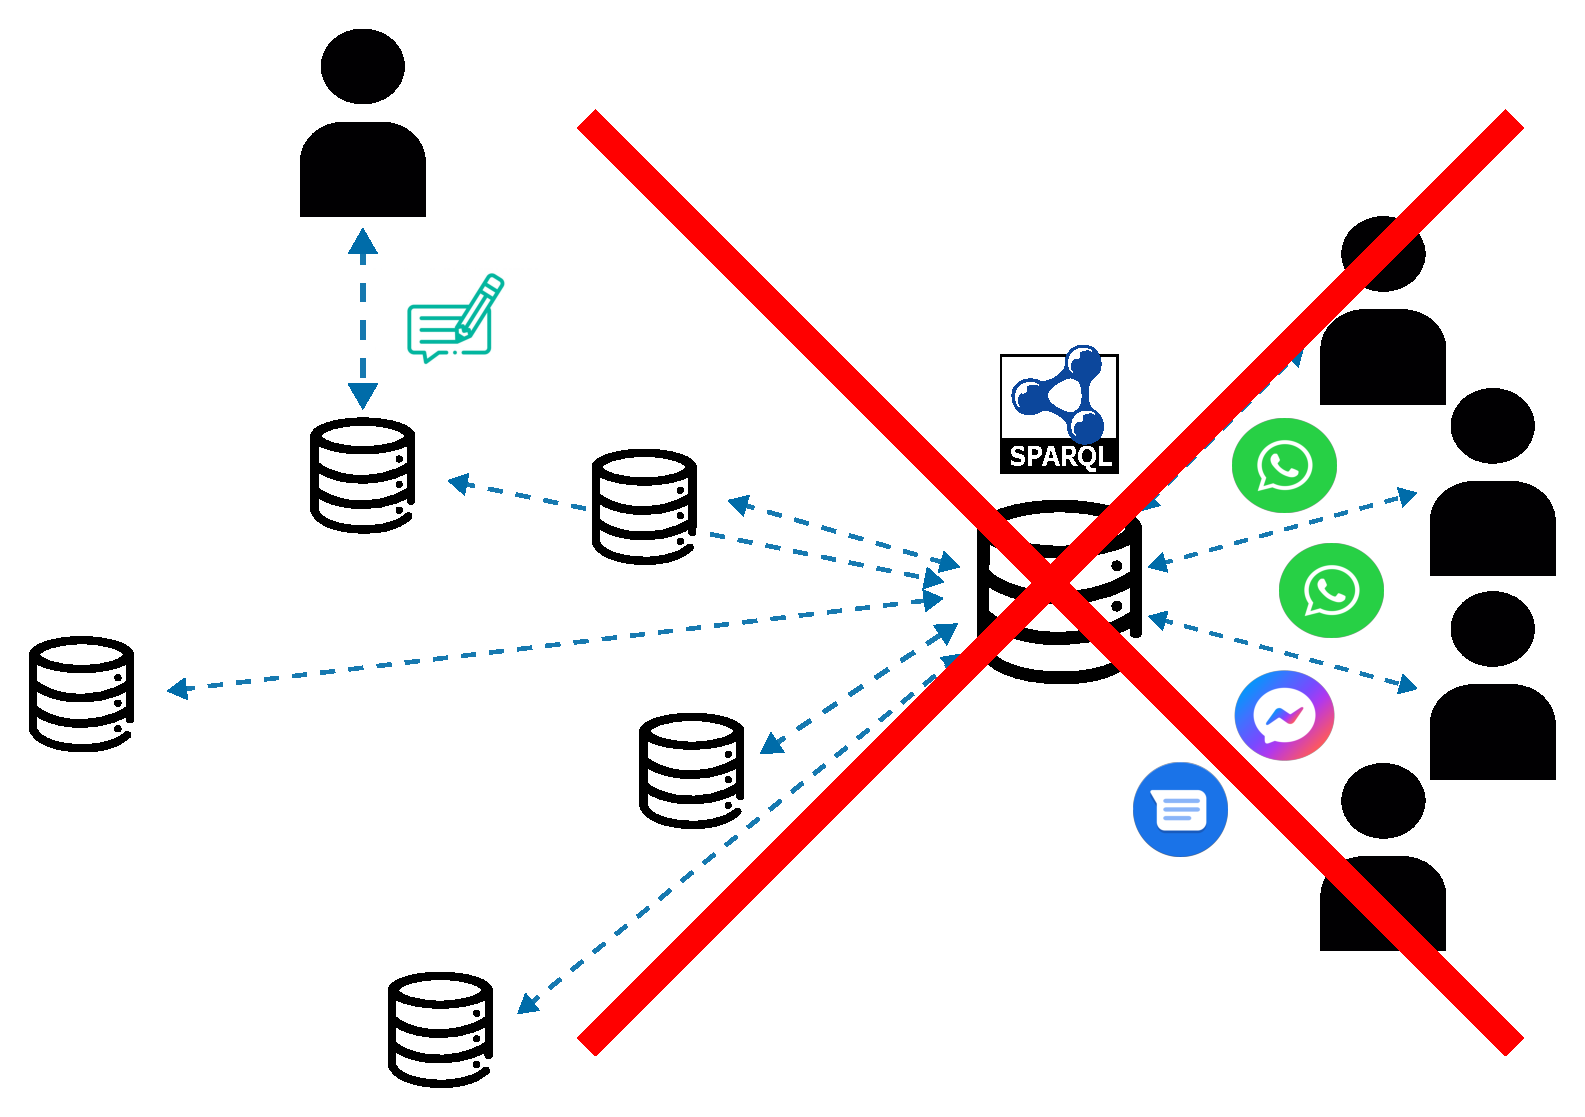
\includegraphics[width=\linewidth]{images/centralize-personal-data-stores-no.pdf} % replace with your image file
        \end{column}

        % Right column: Text
        \begin{column}{0.4\textwidth} % Adjust width as needed
            \begin{itemize}
                \item Why not aggregate data and query it?
                \item Difficult in case of personal data due to privacy concerns
            \end{itemize}
        \end{column}
    \end{columns}
\end{frame}


% \begin{frame}[t]{Link Traversal-based Query Processing}
%     \begin{itemize}
%         \item Link Traversal iteratively dereferences data to query over
%         \item Continuously produces results
%         \item Can enforce fine-grained (document-level) access-control
%     \end{itemize}
% \end{frame}


\begin{frame}{Link Traversal: Seed Document}
    \begin{columns}[T] % T aligns columns at the top
        % Left column: Image
        \begin{column}{0.6\textwidth} % Adjust width as needed
            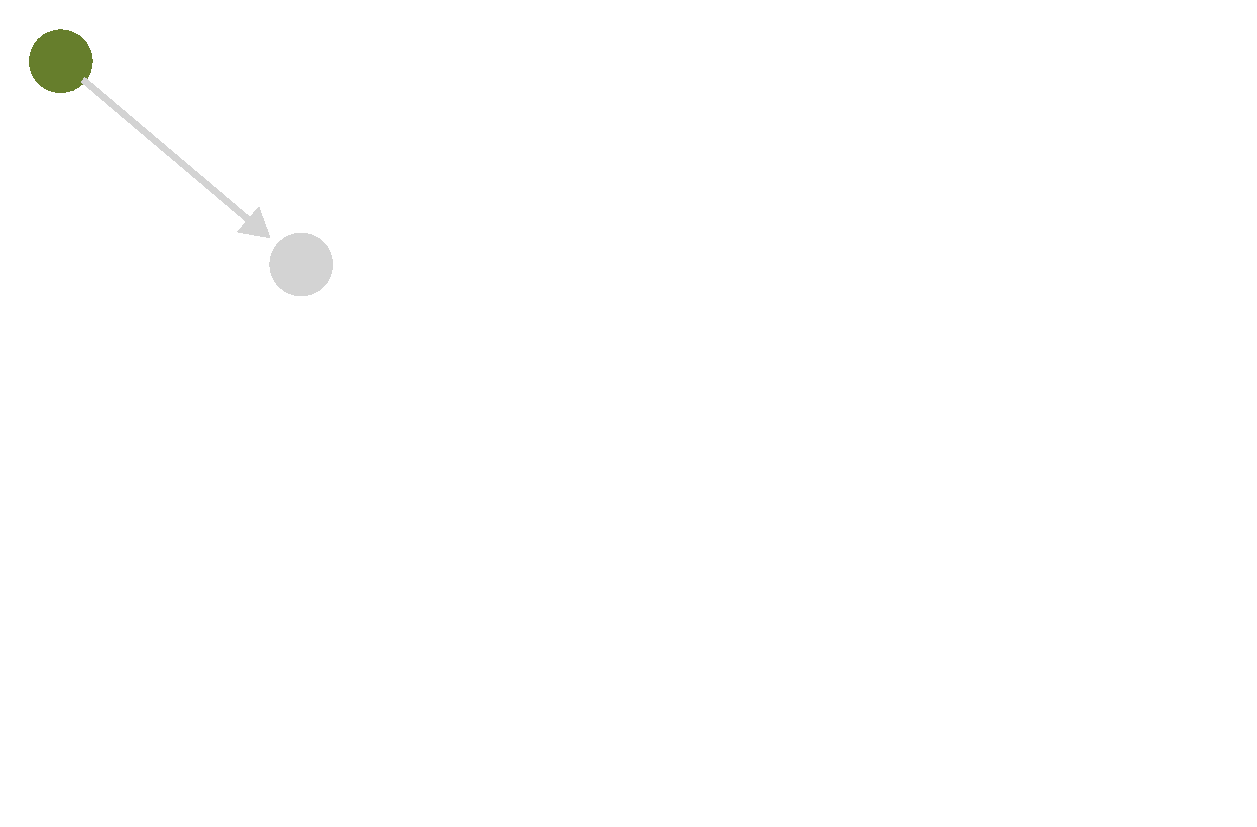
\includegraphics[width=\linewidth]{images/showing-link-traversal-step-0.pdf} % replace with your image file
        \end{column}

        % Right column: Text
        \begin{column}{0.4\textwidth} % Adjust width as needed
            \begin{itemize}
                \item Link Traversal starts from seed documents (URIs)
                \item These are provided by the user or in the query.
            \end{itemize}
        \end{column}
    \end{columns}
\end{frame}

\begin{frame}{Link Traversal: Traversal}
    \begin{columns}[T] % T aligns columns at the top
        % Left column: Image
        \begin{column}{0.6\textwidth} % Adjust width as needed
            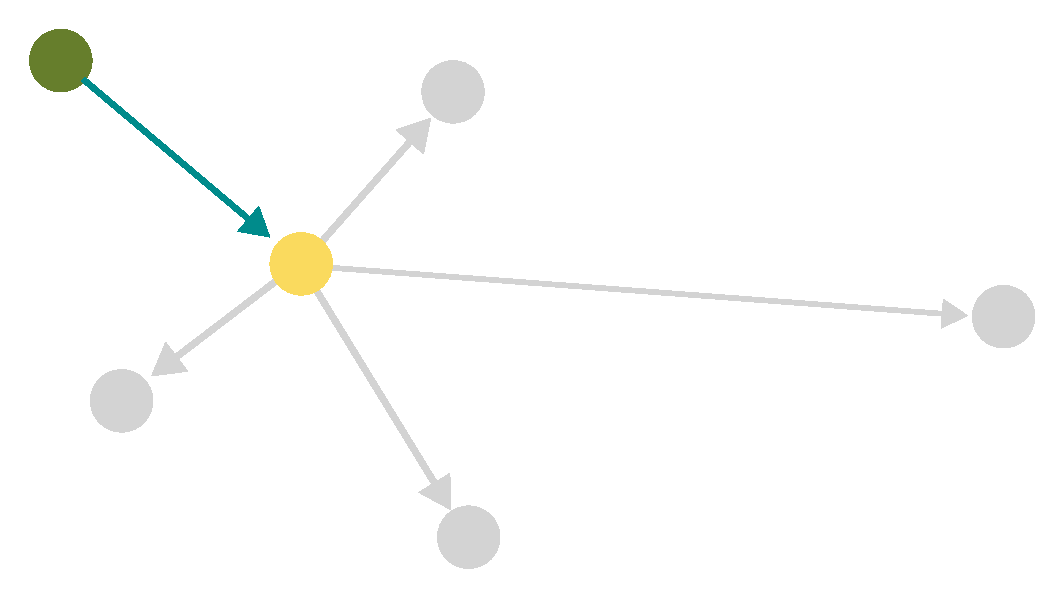
\includegraphics[width=\linewidth]{images/showing-link-traversal-step-1.pdf} % replace with your image file
        \end{column}

        % Right column: Text
        \begin{column}{0.4\textwidth} % Adjust width as needed
            \begin{itemize}
                \item New URIs are extracted from the seed document
                \item URIs are extracted in accordance with reachability criterions
            \end{itemize}
        \end{column}
    \end{columns}
\end{frame}


\begin{frame}{Link Traversal: Traversal}
    \begin{columns}[T] % T aligns columns at the top
        % Left column: Image
        \begin{column}{0.6\textwidth} % Adjust width as needed
            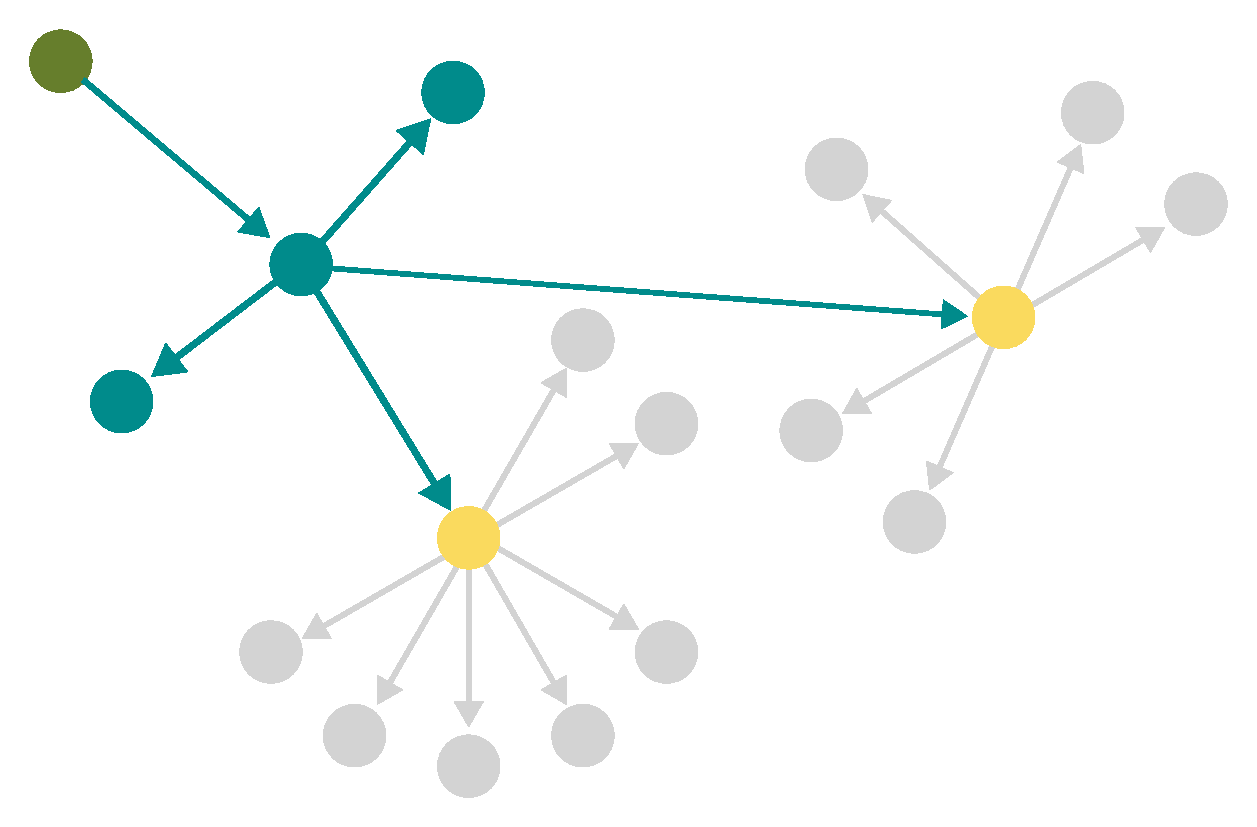
\includegraphics[width=\linewidth]{images/showing-link-traversal-step-2.pdf} % replace with your image file
        \end{column}

        % Right column: Text
        \begin{column}{0.4\textwidth} % Adjust width as needed
            \begin{itemize}
                \item New URIs are dereferenced and the process is repeated
            \end{itemize}
        \end{column}
    \end{columns}
\end{frame}



\begin{frame}{Link Traversal: Termination}
    \begin{columns}[T] % T aligns columns at the top
        % Left column: Image
        \begin{column}{0.6\textwidth} % Adjust width as needed
            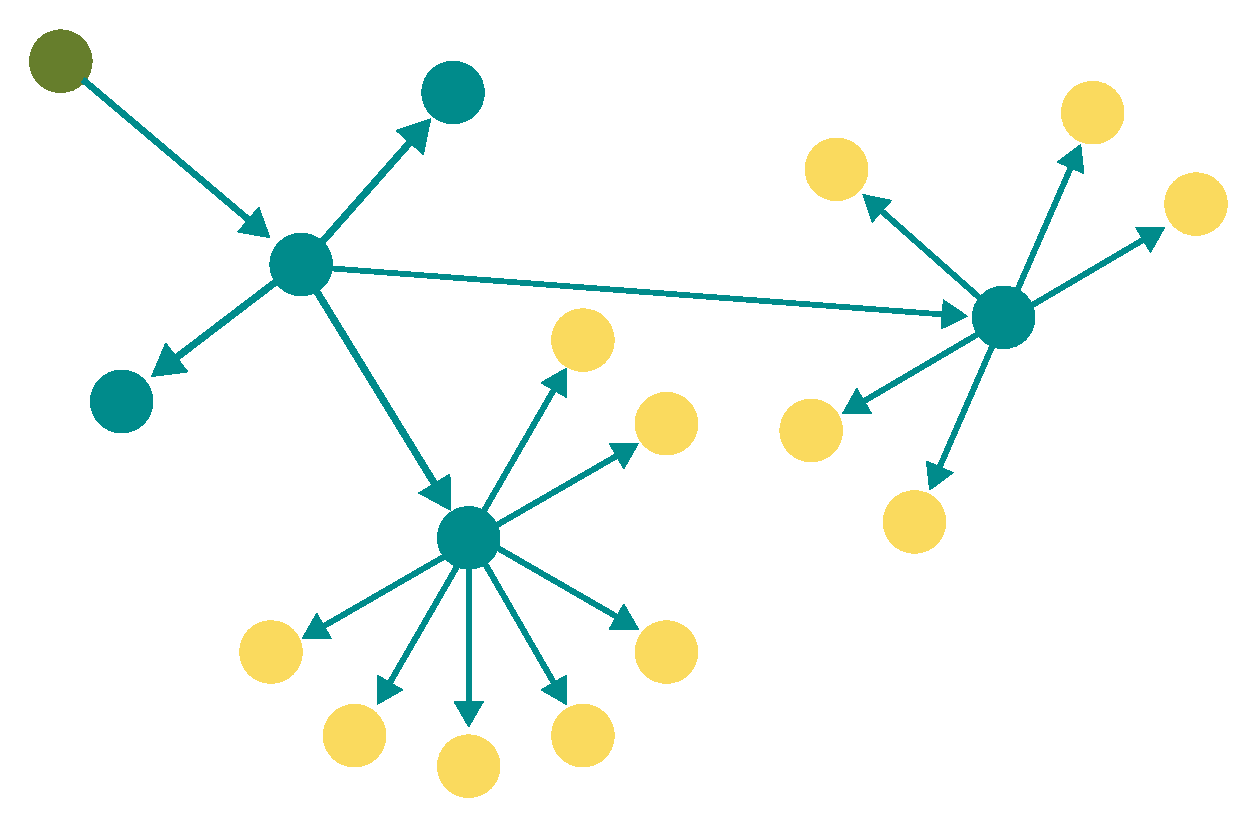
\includegraphics[width=\linewidth]{images/showing-link-traversal-step-3.pdf} % replace with your image file
        \end{column}

        % Right column: Text
        \begin{column}{0.4\textwidth} % Adjust width as needed
            \begin{itemize}
                \item This continues until all links are dereferenced
                \item Continuously produces results
                \item Can enforce fine-grained (document-level) access-control

            \end{itemize}
        \end{column}
    \end{columns}
\end{frame}
\begin{frame}{Query Optimization for Link Traversal}
    \begin{columns}[T] % T aligns columns at the top
        % Left column: Image
        \begin{column}{0.6\textwidth} % Adjust width as needed
            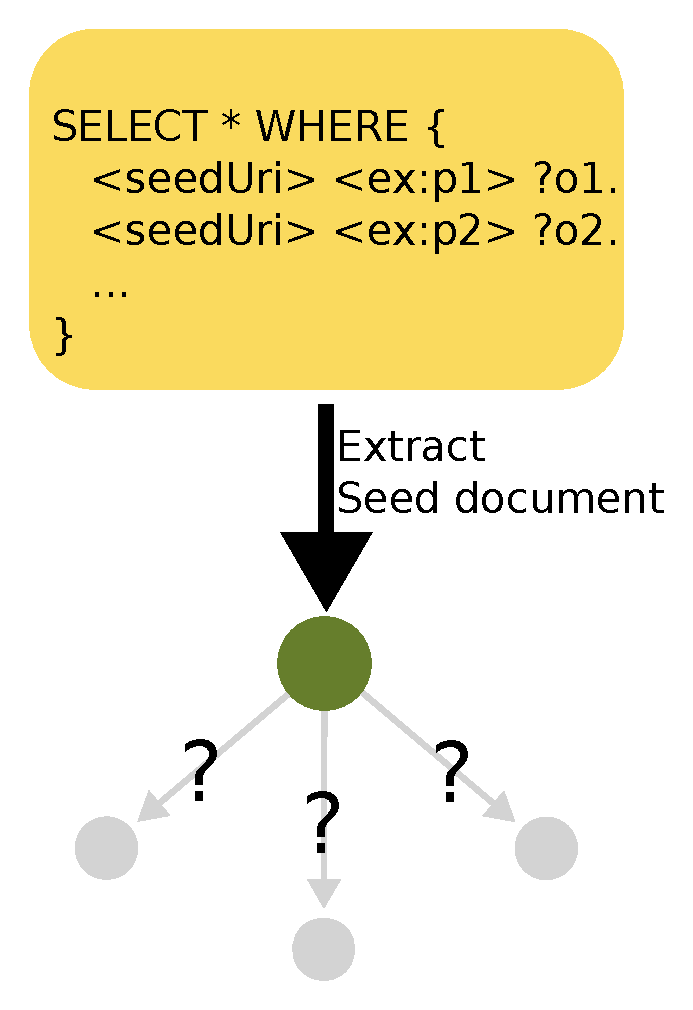
\includegraphics[width=.85\linewidth]{images/hardToOptimizeLTQP.pdf} % replace with your image file
        \end{column}

        % Right column: Text
        \begin{column}{0.4\textwidth}
            The query (partly) determines:
            \begin{itemize}
                \item The queried data
                \item The topology of the queried data
                \item The query-relevant documents
            \end{itemize}
            Result: limited prior knowledge for query optimization
        \end{column}
    \end{columns}
\end{frame}


% NOTES (Done): 
%   - Mention clearly that we introduce is at a research ready tool to analyse prioritization using R3 (Its our new contribution)

\begin{frame}{Problem Statement}
    \centering
    Evaluate the performance of existing link prioritization algorithms in structured decentralized environments
\end{frame}

\begin{frame}{Problem Statement}
    \begin{itemize}
        \item These algorithms are implemented in an engine that is no longer maintained
        \item The baseline performance depends on design choices orthogonal to the prioritization algorithm
        \item The baseline should isolate and measure the marginal effect of the prioritization strategy
    \end{itemize}
\end{frame}


\begin{frame}{$R^{3}$ metric: Motivation}
    \begin{block}{Context}
        During link traversal, the engine traverses a fixed topology entirely
    \end{block}

    \begin{block}{Goal}
        The goal of prioritization is to find query-relevant (\emph{where-provenance}) documents as soon as possible.
    \end{block}

  \begin{alertblock}{Challenge}
        Find the \textbf{optimal traversal order} of a given query in hindsight to compare the traversal order taken by the engine to.
    \end{alertblock}
\end{frame}


\begin{frame}{$R^{3}$ metric: Steiner Trees}
    \begin{itemize}
        \item Directed graph steiner tree over traversed directed graph $G = (V, A)$ with root $r$
        \item Query-relevant documents $D_{T}$ serve as terminals $T \subseteq V$
        \item Find minimum cost sub-graph $X = (V', A')$ starting at root $r$ and spanning all vertexes $T$.
        \item With cost: $ C(X) = \sum\nolimits_{a \in A'} c(a), $, with $c(a)$ the cost of an edge in the topology
    \end{itemize}
\end{frame}


\begin{frame}{$R^{3}$ metric}
  \begin{block}{Definition}
    \[
      R^{3} = \frac{C(X)}{C(O_{\mathcal{T}})}
    \]
  \end{block}

  \begin{itemize}
    \item $X$: the \textbf{optimal traversal order} (minimal-cost path)
    \item $O_{\mathcal{T}}$: traversal order produced by the link prioritization algorithm
    \item $C(\cdot)$: The total cost of all arcs in the traversal path
  \end{itemize}
  \vspace{0.8em}
  \begin{exampleblock}{Interpretation}
    \begin{itemize}
      \item $R^{3} = 1$ → perfect match with the optimal traversal  
      \item $R^{3} < 1$ → deviation from optimal performance  
      \item \textbf{Higher values indicate better prioritization quality.}
    \end{itemize}
  \end{exampleblock}

\end{frame}

\begin{frame}{$R^{3}$ Metric: Introduction}
  \centering
  \begin{columns}[c]
    \column{0.48\textwidth}
    \begin{figure}
      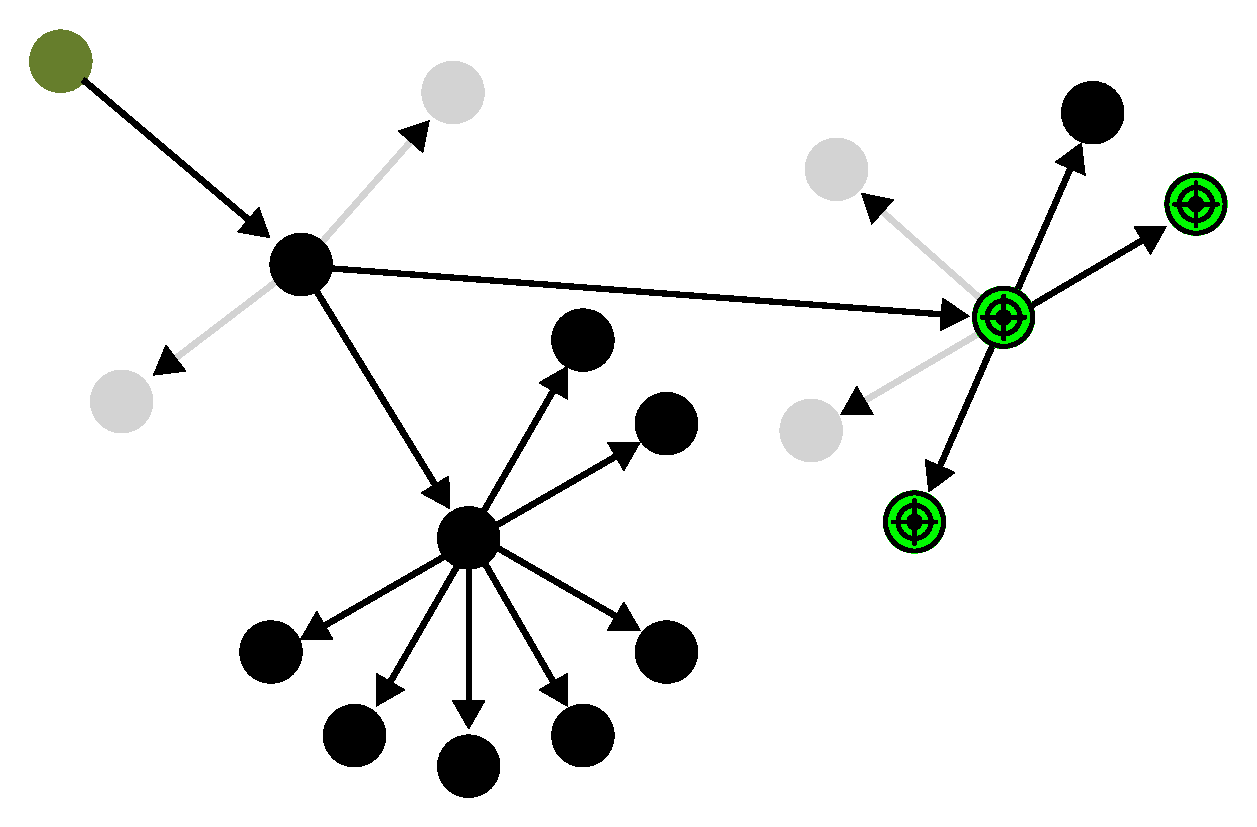
\includegraphics[width=\linewidth]{images/r3-metric-bad-traversal.pdf}
      \caption{\small Actual traversal}
    \end{figure}

    \column{0.48\textwidth}
    \begin{figure}
      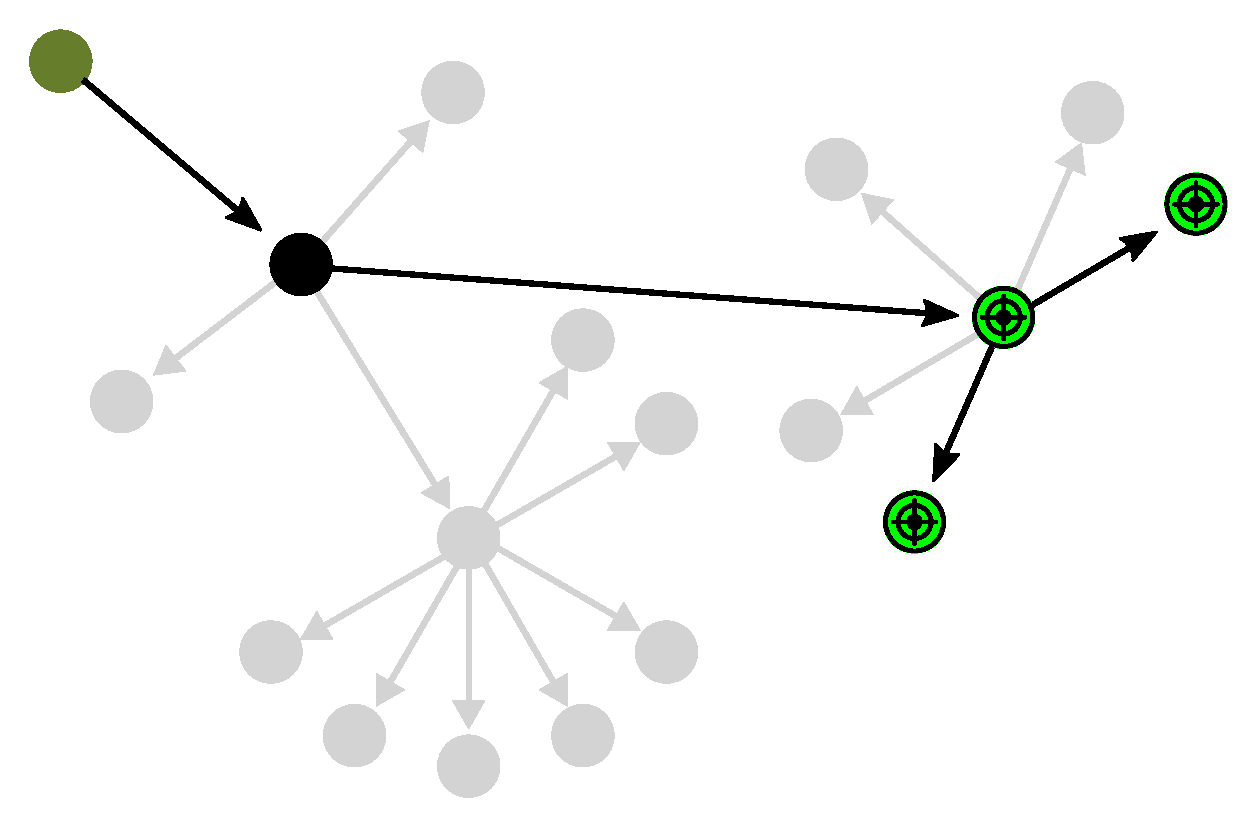
\includegraphics[width=\linewidth]{images/r3-metric-good-traversal.pdf}
      \caption{\small Optimal traversal: minimal cost path}
    \end{figure}
  \end{columns}

  \vspace{1em}
  \small $ R^{3} = \frac{5}{13} = 0.38$
\end{frame}
\begin{frame}{Investigated Structured Decentralized Environment}
  \begin{block}{Simulated Solid Environment: SolidBench \parencite{taelman2023link}}
    \begin{itemize}
        \item Data is stored in vaults simulating social media application
    \end{itemize}
  \end{block}
  \begin{block}{Data attributes}
        \begin{itemize}
            \item Generates 158,233~RDF files 
            \item Across 1,531~data vaults
            \item containing a total of 3,556,159~triples.
    \end{itemize}
  \end{block}
  \begin{block}{Analysed queries}
        \begin{itemize}
        \item Use discover queries
    \end{itemize}
  \end{block}
\end{frame}

% \begin{frame}[t]{Metrics Used}
%     \begin{itemize}
%         \item Time until first result and last result
%         \item Relative to breadth-first traversal baseline
%         \item $R^{3}$
%     \end{itemize}
% \end{frame}


\begin{frame}{Prioritization algorithms}
  \begin{block}{Non-adaptive}
    \begin{itemize}
        \item Breadth-first (default), depth-first, random prioritization
    \end{itemize}
  \end{block}
  \begin{block}{Graph-based}
        \begin{itemize}
        \item In-degree, PageRank score
    \end{itemize}
  \end{block}
  \begin{block}{Result-based}
        \begin{itemize}
        \item Uses result contribution count (RCC) of each node (URI) in the topology
        \item Priority set based on the sum or count of non-zero RCC of the 1 or 2-hop in-neighbours of a node
        \item Called rcc-1, rcc-2, rel-1, rel-2 respectively. 
    \end{itemize}
  \end{block}
\end{frame}

\begin{frame}{Prioritization algorithms}
  \begin{block}{Intermediate-results}
        \begin{itemize}
        \item Uses intermediate solutions in the engine
        \item Priority of URI is determined by the largest intermediate result with that URI bound
        \item \emph{IS} sets initial priorities to 0, while \emph{ISdcr} sets priority to the priority of the parent node - 1
    \end{itemize}
  \end{block}
  \begin{block}{Hybrid}
        \begin{itemize}
        \item Multiply intermediate and full result scoring functions
        \item \emph{is-rcc1}, \emph{is-rcc2}, \emph{is-rel1}, \emph{is-rel2} 
    \end{itemize}
  \end{block}
  \begin{block}{TypeIndex}
        \begin{itemize}
        \item TypeIndex points to location for resource of specific type
        \item Prioritize TypeIndex
    \end{itemize}
  \end{block}
\end{frame}

\begin{frame}[t]{Prioritization algorithms}
  \begin{block}{Oracle}
        \begin{itemize}
        \item Compute RCC in hindsight
        \item Scores are propegated through the shortest path
        \item Serves as optimal performance oracle
    \end{itemize}
  \end{block}
\end{frame}


% \begin{frame}{Prioritization Has Limited Impact on Result Arrival Time}
%   \vspace{-0.5cm}
%   \begin{center}
%     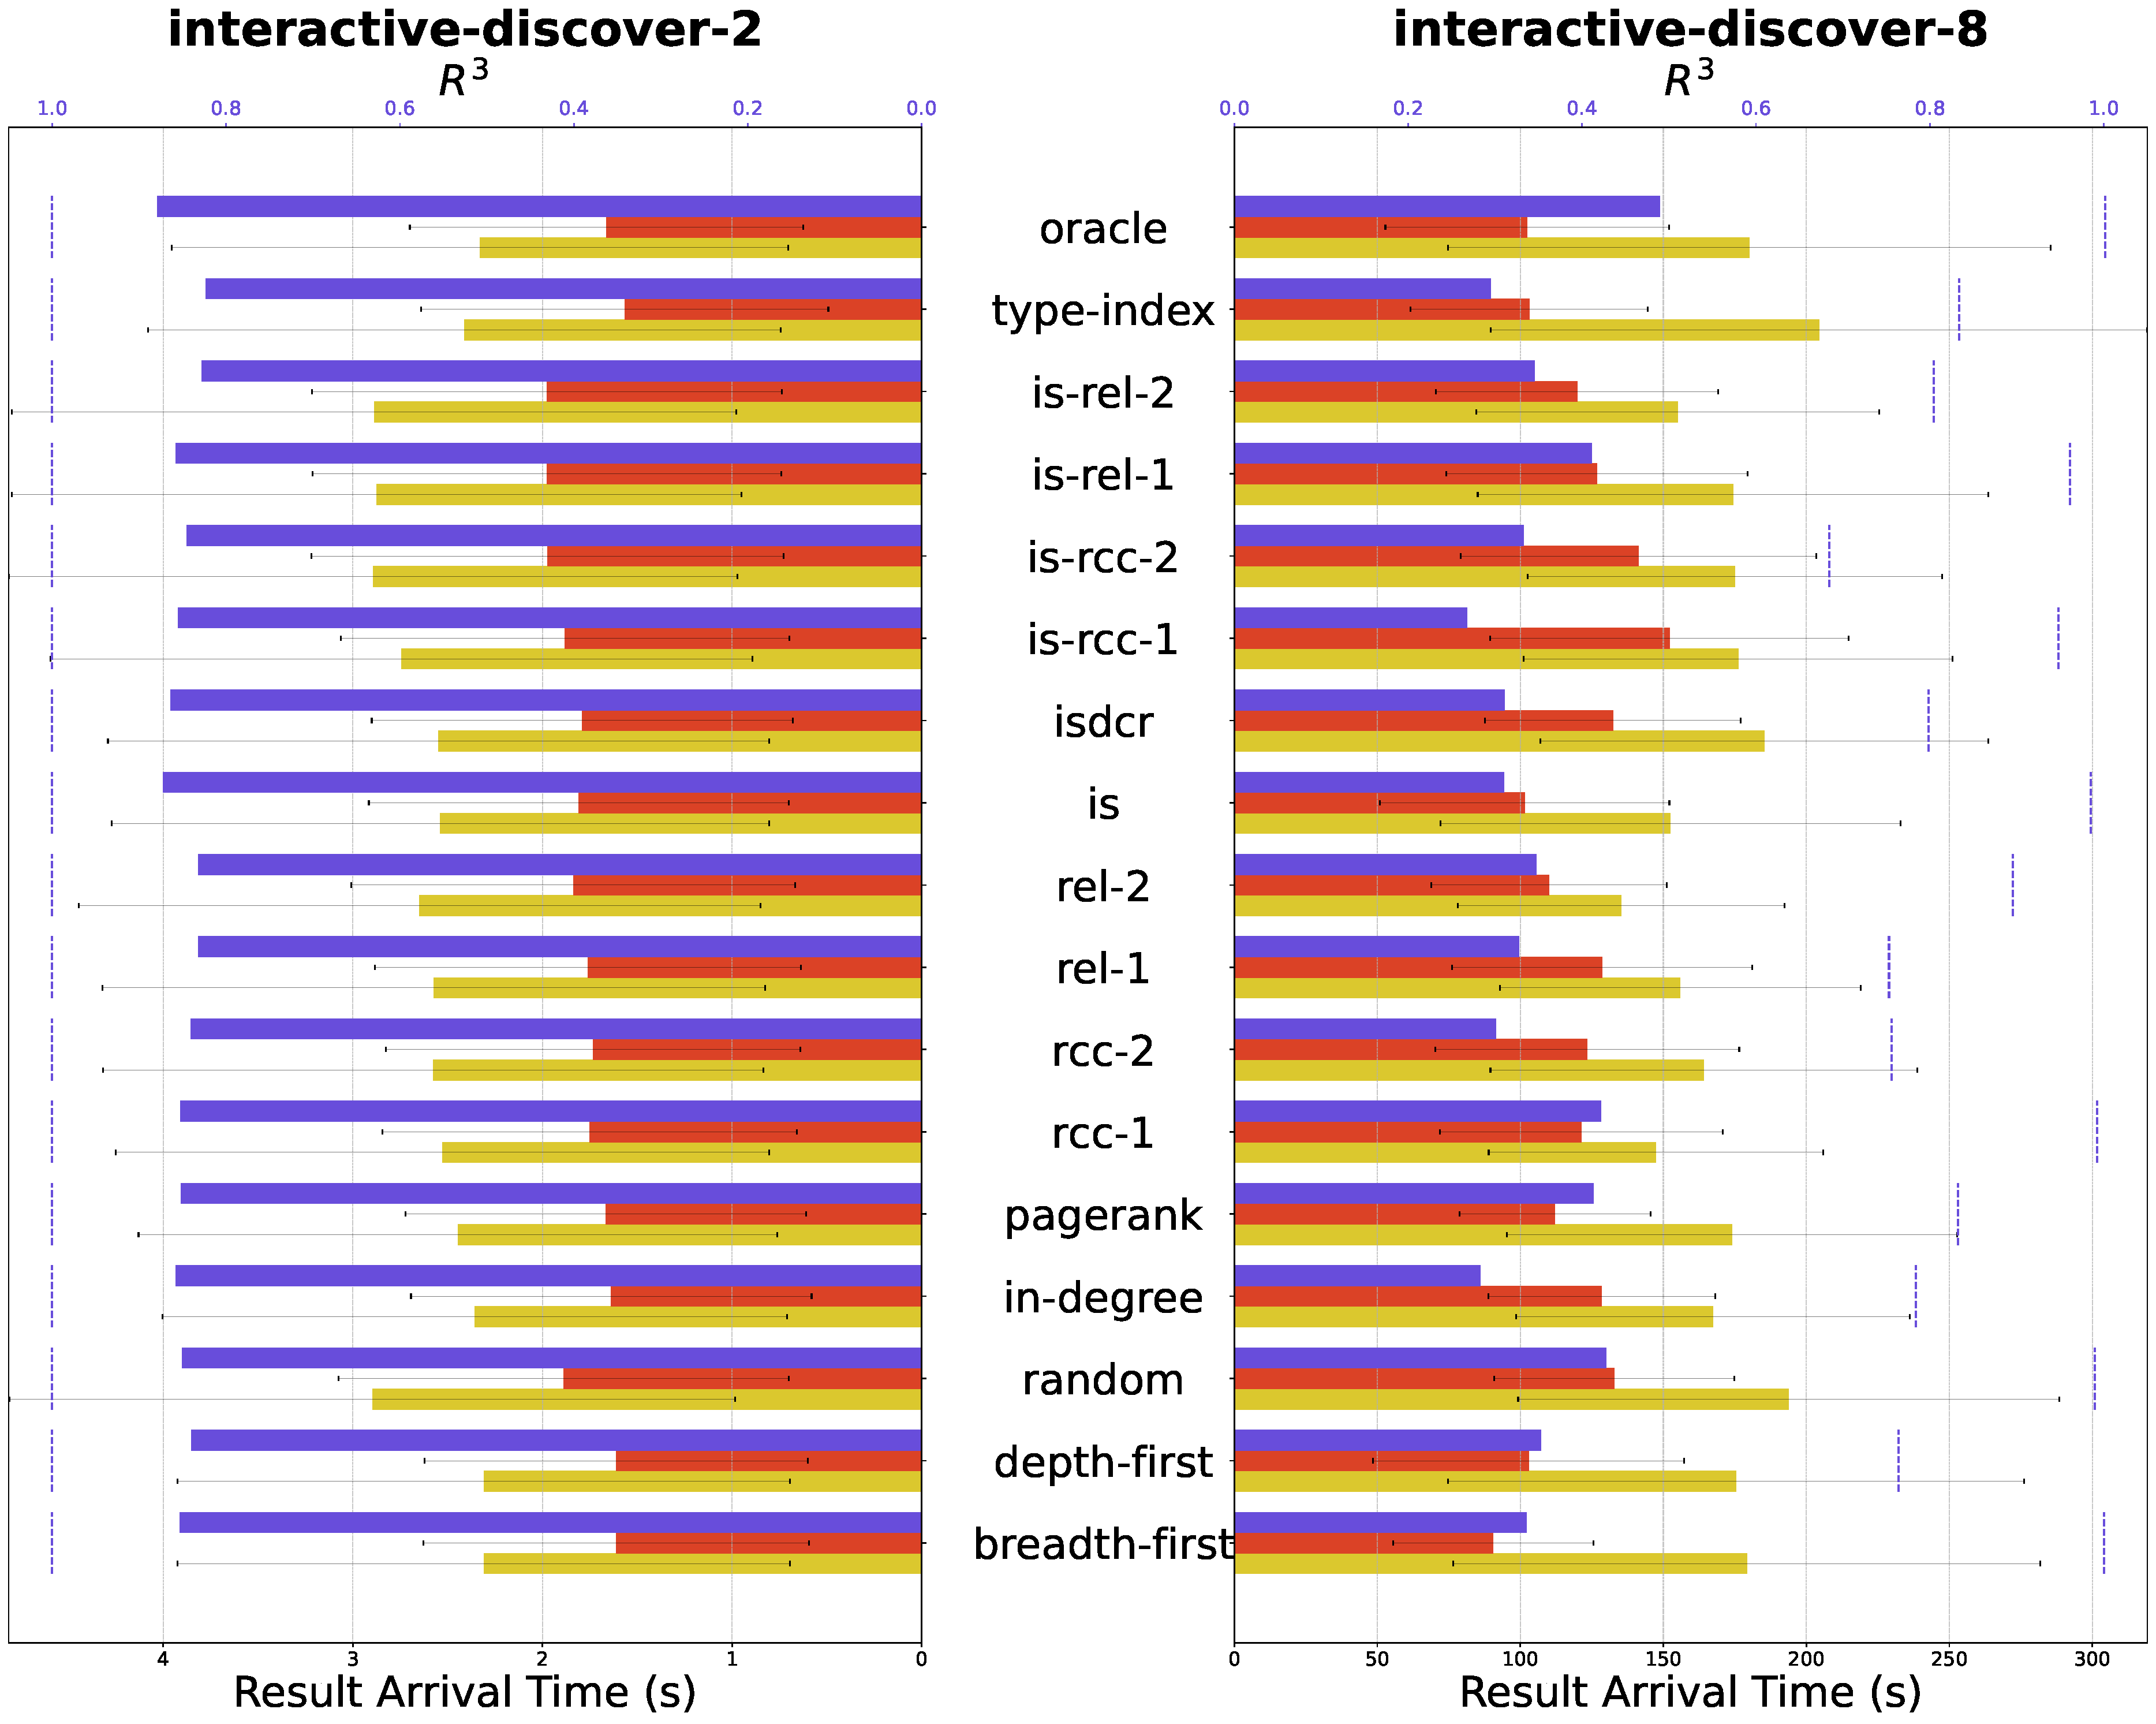
\includegraphics[width=\linewidth,height=0.7\textheight,keepaspectratio]{images/reduced-result-plot-presentation.pdf}
%   \end{center}
%   \vspace{0.3cm}

%   \begin{center}
%     \small
%     \begin{itemize}
%         \item Breadth-first outperforms most algorithms
%         \item Oracle has significantly better $R^{3}$, but not execution time
%     \end{itemize}
%   \end{center}
% \end{frame}

% NOTES: 
%   - FIgure should be entire slide, x / y ticks should be bigger, animation to pop in boxes of text on where to focus and comments on it

\begin{frame}{Prioritization Has Limited Impact on Result Arrival Time}
    \begin{columns}[T] % T aligns columns at the top
        % Left column: Image
        \begin{column}{0.6\textwidth} % Adjust width as needed
            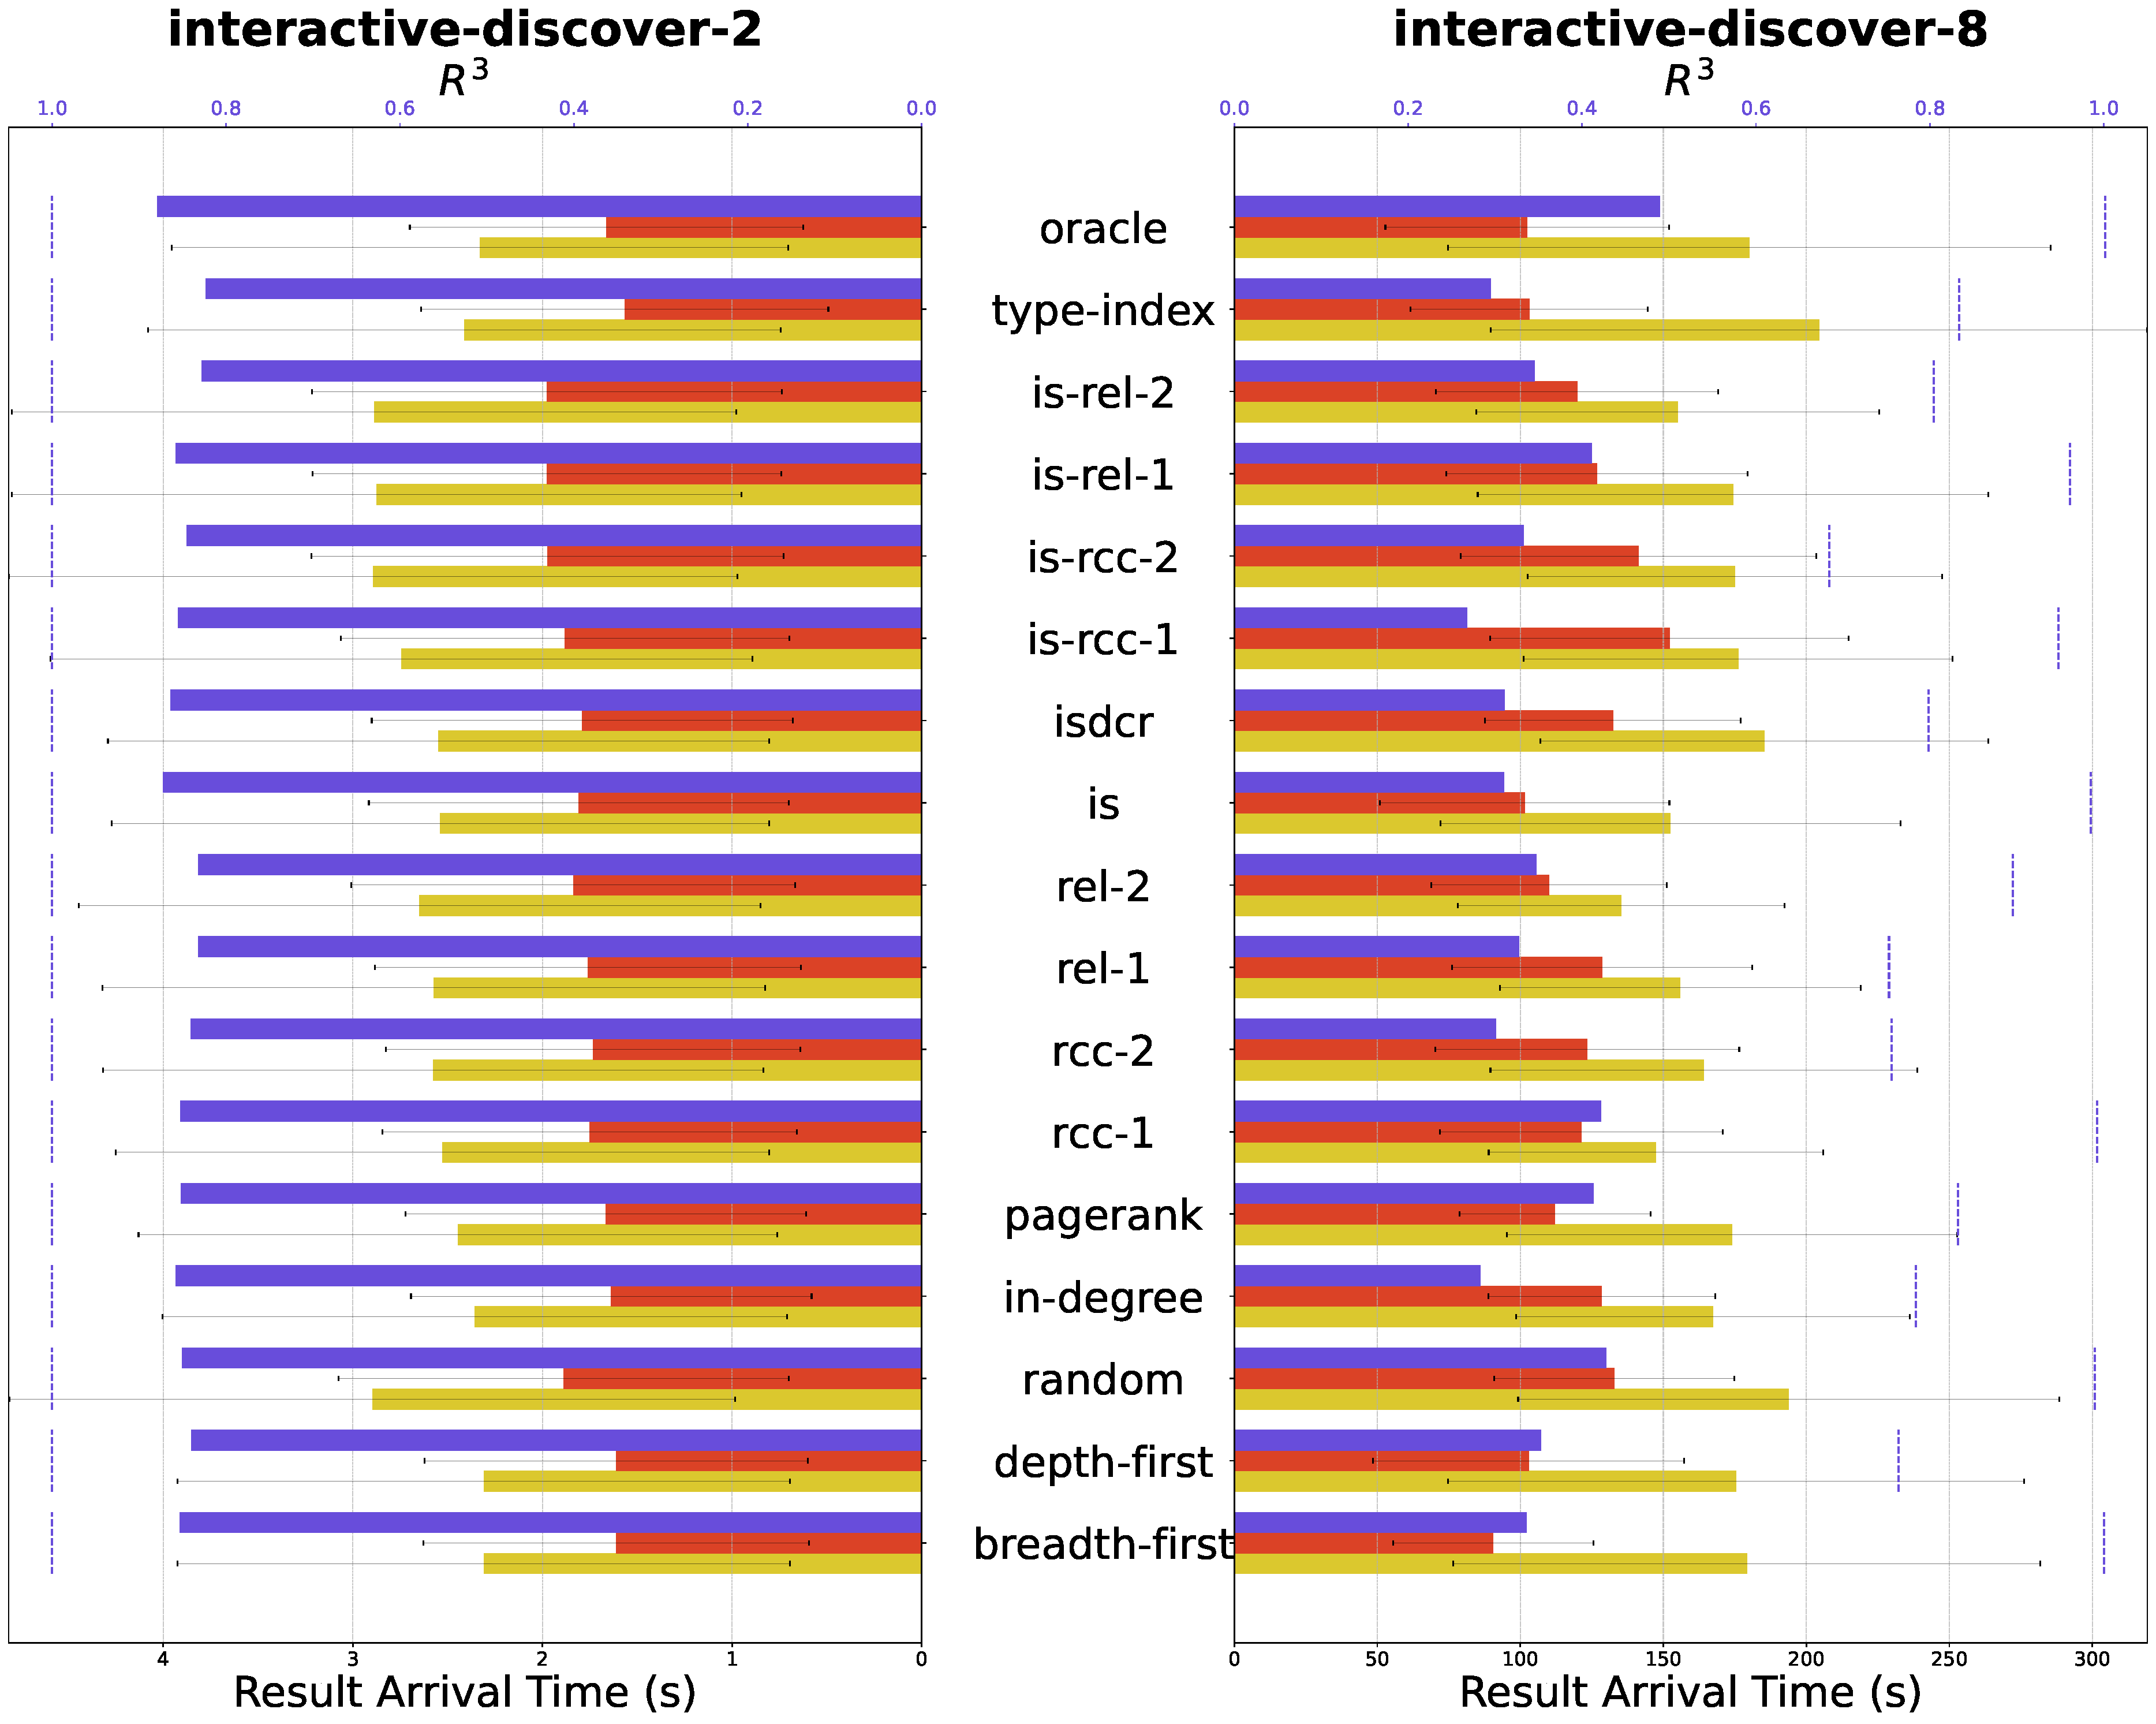
\includegraphics[width=\linewidth]{images/reduced-result-plot-presentation.pdf} % replace with your image file
        \end{column}

        % Right column: Text
        \begin{column}{0.4\textwidth}
          \begin{itemize}
              \item Breadth-first outperforms most algorithms
              \item Oracle has significantly better $R^{3}$, but not execution time
          \end{itemize}
        \end{column}
    \end{columns}
\end{frame}



\begin{frame}{Prioritization Has Limited Impact on Result Arrival Time}
  \small % or \footnotesize, \scriptsize
  \captionsetup[table]{skip=10pt, font=footnotesize }
  \begin{table}[!ht]
    \centering
    \begin{adjustbox}{width=0.9\textwidth} % or e.g., 0.8\textwidth
      \begin{tabular}{l|rr|rr|rr}
        & \multicolumn{2}{c}{$1st$} & \multicolumn{2}{c}{$Cmpl$} & \multicolumn{2}{c}{$R^{3}$} \\
        & better & worse & better & worse & better & worse  \\
        \midrule
        \bf depth-first & \underline{15.7} & \underline{17.1} & \underline{14.3} & 17.1 & 7.5 & 12.5  \\
        \bf random & 4.3 & 68.6 & 5.7 & 74.3 & \underline{15.0} & 15.0 \\
        \hline
        \bf is-rcc-1 & 4.3 & 57.1 & 5.7 & 60.0 & 7.5 & \underline{5.0} \\
        \hline
        \bf type-index & \underline{15.7} & 18.6 & 10.0 & \underline{15.7} & 12.5 & 20.0 \\
        \hline
        \bf oracle & \underline{\underline{\textbf{18.6}}} & \underline{\underline{\textbf{11.4}}} 
        & \underline{\underline{\textbf{18.6}}} & \underline{\underline{\textbf{12.9}}} 
        & \underline{\underline{\textbf{25.0}}} & \underline{\underline{\textbf{2.5}}} \\
      \end{tabular}
    \end{adjustbox}
    \caption{Percentage of queries for which an algorithm performs at least 10\% better or worse than the breadth-first baseline.}
  \end{table}
  \begin{itemize}
    \item No algorithm improves performance, and the oracle only marginally improves performance
  \end{itemize}
\end{frame}
\begin{frame}{Link Prioritization in Structured Decentralized Environments}

    \rule{\linewidth}{0.4pt}

    \textbf{Main takeaway:} Link prioritization has limited performance benefit.

    \vspace{0.6em}
    \begin{itemize}
        \item Limited performance improvement from prioritizing links.
        \item Focus instead on:
        \begin{itemize}
            \item \textbf{Query planning} \textcite{hanski2025link}
            \item \textbf{Traversal pruning} \textcite{tam2024opportunities}
        \end{itemize}
    \end{itemize}

    \rule{\linewidth}{0.4pt}

\end{frame}


% --- Bibliography slide ---
\begin{frame}[allowframebreaks]{References}
  \printbibliography[heading=none]
\end{frame}

% NOTES:
% Supplemental slides:
% 
% Examples of discover, short short, short long, complex queries
% Other metrics, such as diefficiency, weighted R^{3} continuos R^{3}?

\end{document}